\documentclass{beamer}
\usetheme{Darmstadt}

%Temas sin barra de navegación:
%default, boxes, Bergen, Boadilla, Madrid ,
%AnnArbor, CambridgeUS, Pittsburgh, Rochester,
%Temas con barra de navegación tipo árbol:
%Antibes, JuanLesPins
%Temas con tabla de contenidos lateral:
%Berkeley, PaloAlto, Goettingen, Marburg, Hannover
%Temas con navegación en miniframes:
%Berlin, Ilmenau, Dresden, Darmstadt(usado en ésta presentación), Frankfurt, Singapore, Szeged
%Temas con menús de sección y subsección:
%Copenhagen, Luebeck, Malmoe, Warsaw

\usepackage{comment}
\usepackage[utf8]{inputenc}    % Para escribir acentos y caracteres especiales
\usepackage{graphicx}          % Para insertar imágenes
\usepackage{booktabs}          % Para tablas más bonitas
\usepackage{amsmath}           % Para escribir ecuaciones
\usepackage{tikz}              % Para gráficos vectoriales
\usetikzlibrary{calc}          % Para coordenadas calculadas con TikZ
\usepackage{pgfplots}          % Para gráficos matemáticos
\pgfplotsset{compat=1.18}      % Evita errores por compatibilidad
% Comandos personalizados para imprimir números
\usepackage{caption}           % Para mejorar los captions
\usepackage{pgf}               % Para...

\title{Ejemplo completo en Beamer}
\author{Tu Nombre Mateo}
\institute{Tu Institución Udp}
\date{\today}

\begin{document}

% Portada
\begin{frame}
  \titlepage
  \centering \includegraphics[width=3cm]{imagenes/logo.png}
  \end{frame}

% Tabla de contenidos
\begin{frame}
  \frametitle{Contenido}
  \tableofcontents
\end{frame}

\section{Ecuaciones}

% Ejemplo ecuaciones
\begin{frame}
  \frametitle{Ecuación simple}
  Una fórmula conocida:
  \[
    E = mc^2
  \]

  Otra ecuación inline: \( a^2 + b^2 = c^2 \)
\end{frame}

\section{Imágenes}

% Gráfico gspc vs estrategias
\begin{frame}
  \frametitle{Imagen de ejemplo}
  \begin{figure}
    \centering
    \includegraphics[width=0.8\linewidth]{imagenes/Grafico1.png}
    \caption{Un gráfico de ejemplo}
  \end{figure}
\end{frame}

\section{Tablas}

% Tabla de datos
\begin{frame}
  \frametitle{Tabla de datos}
  \begin{table}
    \centering
    \begin{tabular}{lcc}
      \toprule
      Elemento & Valor & Unidades \\
      \midrule
      Hierro (Fe) & 56.0 & g/mol \\
      Cobre (Cu) & 63.5 & g/mol \\
      Zinc (Zn) & 65.4 & g/mol \\
      \bottomrule
    \end{tabular}
    \caption{Ejemplo de tabla con datos químicos}
  \end{table}
\end{frame}

% Tabla de nombres
\begin{frame}
    \frametitle{Tabla de nombres}
    \begin{flushright}
        
        \begin{tabular}{|l|c|r|}
            \hline
            Nombre & Edad & Nota \\
            \hline
            Ana    & 22   & 18.5 \\
            Luis   & 24   & 17.8 \\
            \hline
        \end{tabular}
    \end{flushright}
\end{frame}

% Tabla de cantidades
\begin{frame}
    \title{Tabla de cantidades}
    \begin{flushleft}
        
        \begin{tabular}{|p{4cm}|c|}
            \hline
            Descripción del ítem & Cantidad \\
            \hline
            Esto es un texto largo que se ajusta & 5 \\
            \hline
        \end{tabular}
    \end{flushleft}
\end{frame}

\section{Gráficos con TikZ}

% Gráficos ecuaciones X^2/N
\begin{frame}
  \frametitle{Gráfico con TikZ}
  \begin{tikzpicture}[ scale=.8]
    \draw[->] (-0.5,0) -- (4.5,0) node[right] {x};
    \draw[->] (0,-0.5) -- (0,4.5) node[above] {y};
    \draw[blue, thick, domain=0:4] plot (\x, {\x*\x/4}) node[right] {$y = \frac{x^2}{4}$};
  \end{tikzpicture}
  \begin{tikzpicture}[ scale=.8]
        \draw[->] (-1,0) -- (5,0) node[right] {x};  % Eje X
        \draw[->] (0,-1) -- (0,5) node[above] {y};  % Eje Y
        \draw[domain=0:4, blue, thick] plot (\x, {\x*\x/2}) node[right] {$y = \frac{x^2}{2}$};
      \end{tikzpicture}
\end{frame}

%C írculo y triángulo 
\begin{frame}
    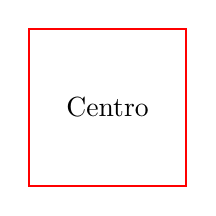
\begin{tikzpicture}
        \draw[red, thick] (0,0) rectangle (2,2);          % Cuadrado
        \node at (1,1) {Centro};                         % Texto en el centro
      \end{tikzpicture}
    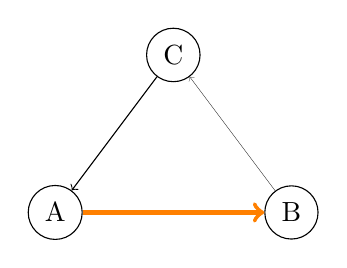
\begin{tikzpicture}
        \node (A) at (0,0) [circle, draw] {A};
        \node (B) at (3,0) [circle, draw] {B};
        \node (C) at (1.5,2) [circle, draw] {C};
      
        \draw[ultra thick,->, orange] (A) -- (B);
        \draw[ultra thin,->] (B) -- (C);
        \draw[->] (C) -- (A);
    \end{tikzpicture}
\end{frame}

% Organigrama empresarial
\begin{frame}
  \frametitle{Organigrama empresarial}
  \begin{figure}
    \resizebox{\linewidth}{!}{
    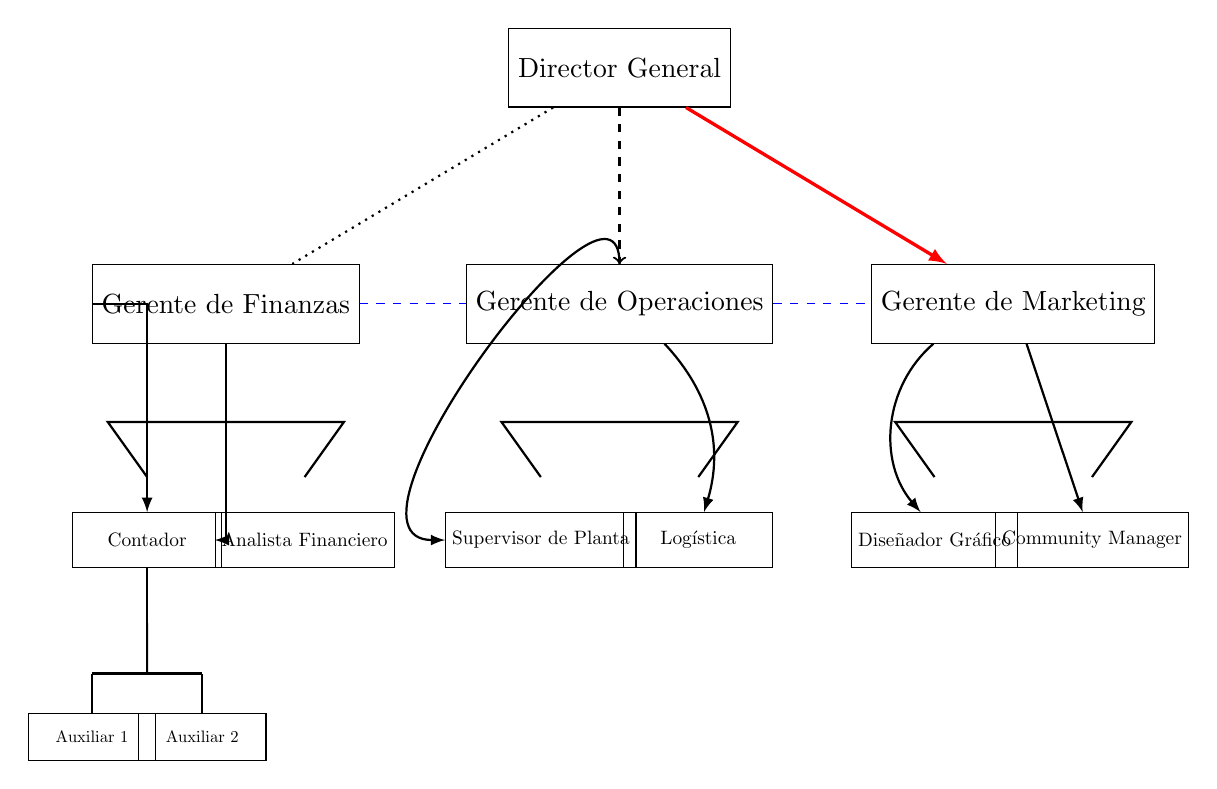
\begin{tikzpicture}[
        every node/.style={rectangle, draw, align=center, minimum width=2.7cm, minimum height=1cm},
        node distance=2cm
        ]
        % Nodos principales
        \node (director) at (0,0) {Director General};
        \node (finanzas) at (-5,-3) {Gerente de Finanzas};
        \node (operaciones) at (0,-3) {Gerente de Operaciones};
        \node (marketing) at (5,-3) {Gerente de Marketing};
        
        % Nodos secundarios
        \node[scale=0.7] (fin1) at (-6,-6) {Contador};
        \node[scale=0.7] (fin2) at (-4,-6) {Analista Financiero};
        
        \node[scale=0.7] (ope1) at (-1,-6) {Supervisor de Planta};
        \node[scale=0.7] (ope2) at (1,-6) {Logística};
        
        \node[scale=0.7] (mkt1) at (4,-6) {Diseñador Gráfico};
        \node[scale=0.7] (mkt2) at (6,-6) {Community Manager};
        
        % Nuevos nodos auxiliares
        \node[scale=0.6] (aux1) at (-6.7,-8.5) {Auxiliar 1};
        \node[scale=0.6] (aux2) at (-5.3,-8.5) {Auxiliar 2};
        
        % Conexiones
        \draw[-, dotted,thick] (director) -- (finanzas);
        \draw[->, dashed, thick] (director) -- (operaciones);
        \draw[-latex,red, very thick] (director) -- (marketing);
        
        \draw[-,dashed,blue] (finanzas)--(operaciones)--(marketing);

        \draw[-latex, thick] (finanzas)  -| (fin1);
        \draw[-latex, thick] (finanzas) |- (fin2);
        % Bifurcación ortogonal desde Contador
        \draw[thick] (fin1.south) -- ++(0,-0.7) coordinate (finaux);
        \draw[thick] (aux1.north) -- ++(0,0.5) coordinate (aux1top);
        \draw[thick] (aux2.north) -- ++(0,0.5) coordinate (aux2top);
        \draw[thick] (aux1top) -- (aux2top);
        \draw[thick] (finaux) -- ($(aux1top)!0.5!(aux2top)$);
        \draw[-latex, thick] (operaciones) to [out=90, in=180] (ope1);
        \draw[-latex, bend left, thick] (operaciones) to (ope2);
        \draw[-latex, bend right=45, thick] (marketing) to (mkt1);
        \draw[-latex, thick] (marketing) -- (mkt2);
        
        % Unión tipo corchete recto por grupo
        \draw[thick] (-6,-5.2) -- (-6.5,-4.5) -- (-3.5,-4.5) -- (-4,-5.2); % Finanzas
        \draw[thick] (-1,-5.2) -- (-1.5,-4.5) -- (1.5,-4.5) -- (1,-5.2);   % Operaciones
        \draw[thick] (4,-5.2) -- (3.5,-4.5) -- (6.5,-4.5) -- (6,-5.2);     % Marketing
        \end{tikzpicture}
    }
  \end{figure}
\end{frame}

% Árbol binomial
\begin{frame}
  \frametitle{Árbol binomial de decisión}
  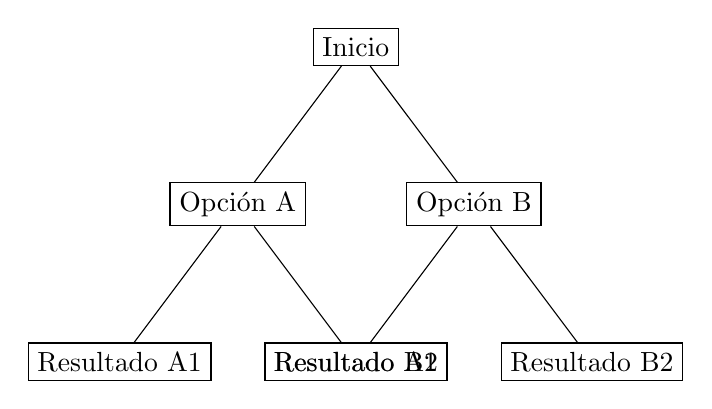
\begin{tikzpicture}[sibling distance=3cm, level distance=2cm,
    every node/.style = {shape=rectangle, draw, align=center}]
    \node {Inicio}
      child {node {Opción A}
        child {node {Resultado A1}}
        child {node {Resultado A2}}
      }
      child {node {Opción B}
        child {node {Resultado B1}}
        child {node {Resultado B2}}
      };
  \end{tikzpicture}
\end{frame}

\section{Colores}

% Cuadros rgb
\begin{frame}
  \frametitle{Ejemplo con colores RGB}
  
\begin{tikzpicture}
    % Rectángulo rojo RGB
    \definecolor{myred}{RGB}{255,0,0}
    \fill[myred] (0,0) rectangle (2,1);
    \node at (1,0.5) {Rojo};

    % Rectángulo verde RGB
    \definecolor{mygreen}{RGB}{0,255,0}
    \fill[mygreen] (2.5,0) rectangle (4.5,1);
    \node at (3.5,0.5) {Verde};

    % Rectángulo azul RGB
    \definecolor{myblue}{RGB}{0,0,255}
    \fill[myblue] (5,0) rectangle (7,1);
    \node at (6,0.5) {Azul};
  \end{tikzpicture}
\end{frame}

% Cuadros superpuestos 
\begin{frame}
    \frametitle{Ejemplo con minipage: Relleno semitransparente}
    \begin{minipage}{\linewidth}
      \centering
      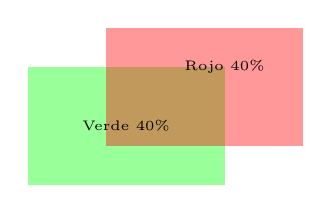
\begin{tikzpicture}
        \fill[green, fill opacity=0.4] (0,0) rectangle (2.5,1.5);
        \fill[red, fill opacity=0.4] (1,0.5) rectangle (3.5,2);
        \node at (1.25,0.75) {\tiny Verde 40\%};
        \node at (2.5,1.5) {\tiny Rojo 40\%};
      \end{tikzpicture}
      \captionof{figure}{Superposición de colores con \texttt{fill opacity}}
    \end{minipage}
\end{frame}

% Cuadro semi transparente
\begin{frame}
  \frametitle{Ejemplo con degradado lineal}
  \begin{minipage}{\linewidth}
    \centering
    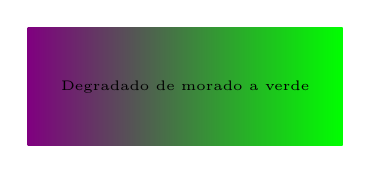
\begin{tikzpicture}
      \shade[left color=violet, right color=green] (0,0) rectangle (4,1.5);
      \node at (2,0.75) {\tiny Degradado de morado a verde};
    \end{tikzpicture}
    \captionof{figure}{Degradado lineal horizontal}
    \frametitle{Ejemplo con minipage: Relleno semitransparente}
        \end{minipage}
\end{frame}
      
% Círculo degradado
\begin{frame}
  \frametitle{Ejemplo con degradado radial}
  \begin{minipage}{\linewidth}
    \centering
    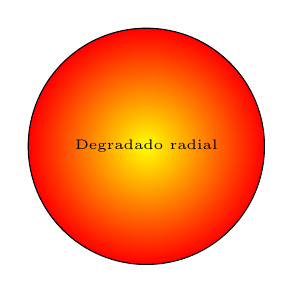
\begin{tikzpicture}
      \shadedraw[inner color=yellow, outer color=red, draw=black] (0,0) circle (1.5cm);
      \node at (0,0) {\tiny Degradado radial};
    \end{tikzpicture}
    \captionof{figure}{Degradado radial del centro hacia afuera}
  \end{minipage}
\end{frame}

% Triangulo con flechas cym
\begin{frame}
  \frametitle{Gráfico con flechas de colores RGB}
  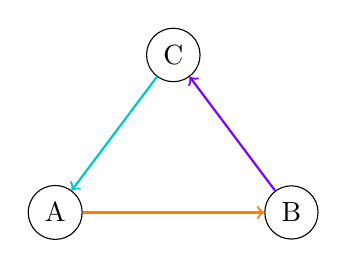
\begin{tikzpicture}
    \definecolor{rgb1}{RGB}{255,128,0}   % Naranja
    \definecolor{rgb2}{RGB}{128,0,255}   % Púrpura
    \definecolor{rgb3}{RGB}{0,200,200}   % Cian

    \node (A) at (0,0) [circle, draw] {A};
    \node (B) at (3,0) [circle, draw] {B};
    \node (C) at (1.5,2) [circle, draw] {C};

    \draw[->, thick, rgb1] (A) -- (B);
    \draw[->, thick, rgb2] (B) -- (C);
    \draw[->, thick, rgb3] (C) -- (A);
  \end{tikzpicture}
\end{frame}

\section{Gráficos con PGFPlots}

% Gráfico Sin(x)
\begin{frame}
  \frametitle{Gráfico PGFPlots}
  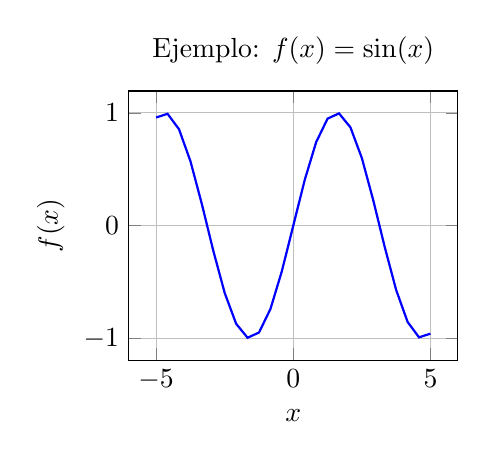
\begin{tikzpicture}
    \begin{axis}[
      width=6.5cm, scale=0.85, clip=true,
      xlabel={$x$},
      ylabel={$f(x)$},
      title={Ejemplo: $f(x)=\sin(x)$},
      grid=major,
    ]
      \addplot[blue, thick] {sin(deg(x))};
    \end{axis}
  \end{tikzpicture}
\end{frame}

% Gráfico X^2
\begin{frame}
  \frametitle{Gráfico de una función cuadrática}
  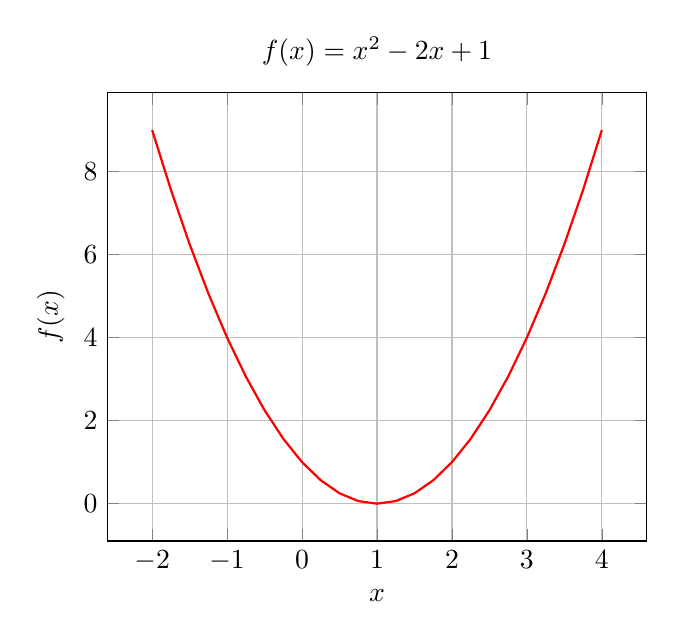
\begin{tikzpicture}
    \begin{axis}[
      xlabel={$x$},
      ylabel={$f(x)$},
      title={$f(x) = x^2 - 2x + 1$},
      grid=both,
    ]
      \addplot[red, thick, domain=-2:4] {x^2 - 2*x + 1};
    \end{axis}
  \end{tikzpicture}
\end{frame}

% Gráfico dispersión
\begin{frame}
  \frametitle{Gráfico de dispersión de puntos}
  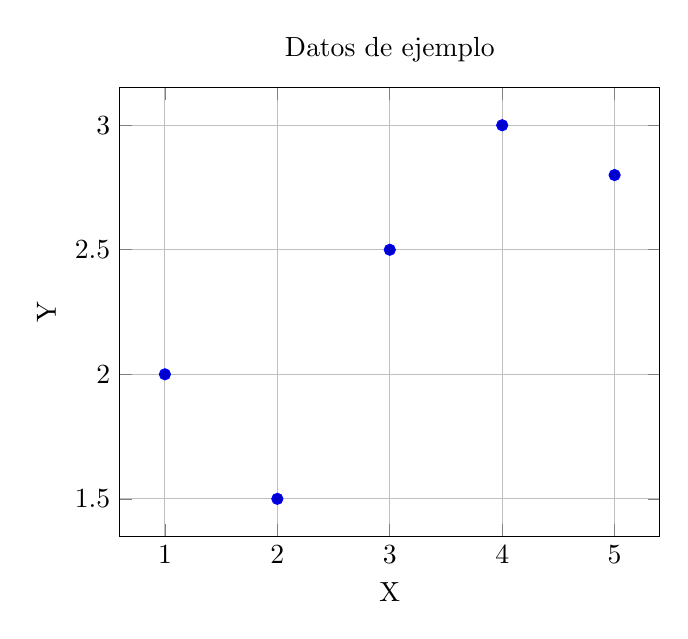
\begin{tikzpicture}
    \begin{axis}[
      xlabel={X},
      ylabel={Y},
      title={Datos de ejemplo},
      only marks,
      grid=major,
    ]
      \addplot coordinates {
        (1,2) (2,1.5) (3,2.5) (4,3) (5,2.8)
      };
    \end{axis}
  \end{tikzpicture}
\end{frame}

% Gráfico doble curva
\begin{frame}
  \frametitle{Gráfico con dos curvas}
  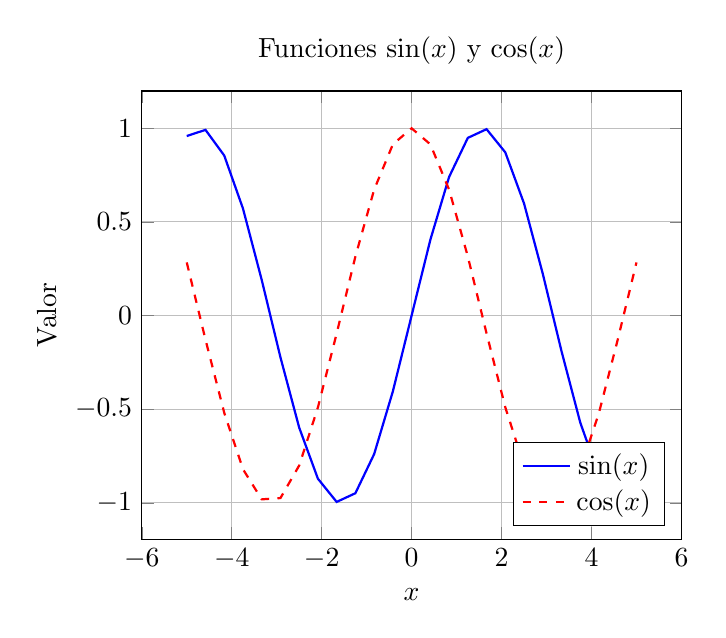
\begin{tikzpicture}
    \begin{axis}[
      xlabel={$x$},
      ylabel={Valor},
      title={Funciones $\sin(x)$ y $\cos(x)$},
      legend pos=south east,
      grid=major,
    ]
      \addplot[blue, thick] {sin(deg(x))};
      \addlegendentry{$\sin(x)$}
      
      \addplot[red, dashed, thick] {cos(deg(x))};
      \addlegendentry{$\cos(x)$}
    \end{axis}
  \end{tikzpicture}
\end{frame}

% Histograma con fuente
\begin{frame}
  \frametitle{Histograma de ejemplo}
  \begin{minipage}{.8 \linewidth}
    \centering
    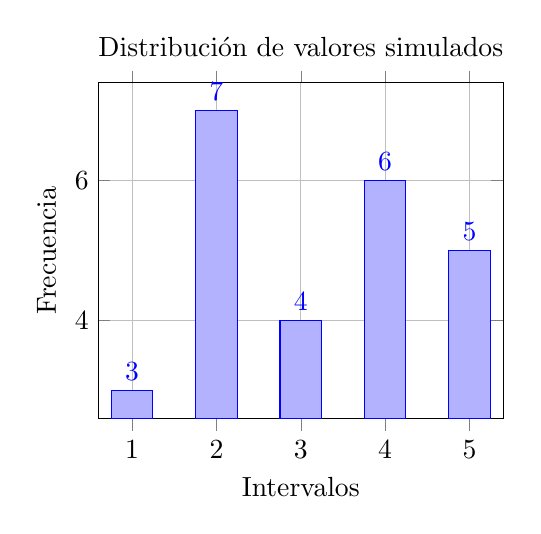
\begin{tikzpicture}
      \begin{axis}[
        ybar,
        xlabel={Intervalos},
        ylabel={Frecuencia},
        title={Distribución de valores simulados},
        xtick=data,
        bar width=15pt,
        nodes near coords,
        grid=major, 
        scale=.75
      ]
        \addplot coordinates {(1,3) (2,7) (3,4) (4,6) (5,5)};
      \end{axis}
    \end{tikzpicture}
    \captionof{figure}{Histograma de valores simulados}
    {\footnotesize Fuente: Elaboración Propia | Datos: \textasciicircum VIX (Yahoo Finance)}
  \end{minipage}
\end{frame}
% Mapa de calor
\begin{frame}
    \frametitle{Mapa de calor}
    {\tiny
    \begin{minipage}{\linewidth}
      \centering
      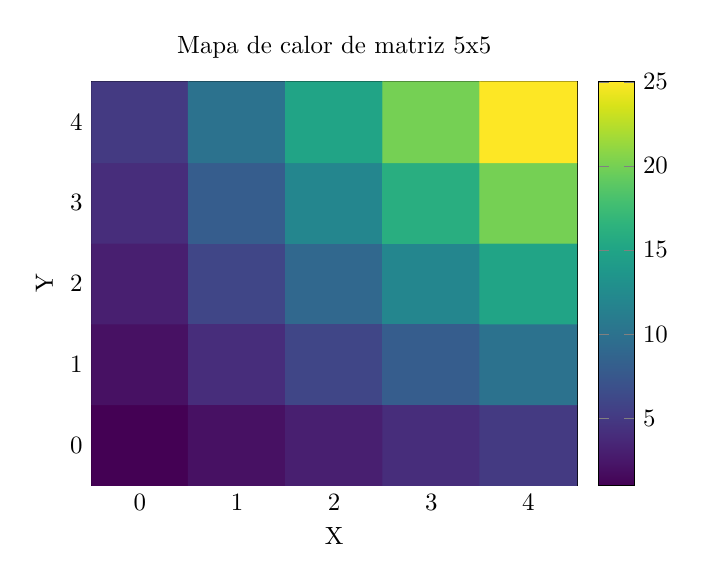
\begin{tikzpicture}[scale=0.9, transform shape]
      \begin{axis}[
          view={0}{90},
          colormap/viridis,
          colorbar,
          xlabel={X},
          ylabel={Y},
          title={Mapa de calor de matriz 5x5},
          mesh/cols=5,
          enlargelimits=false
        ]
          \addplot[matrix plot*, point meta=explicit] coordinates {
            (0,0) [1] (1,0) [2] (2,0) [3] (3,0) [4] (4,0) [5]
            (0,1) [2] (1,1) [4] (2,1) [6] (3,1) [8] (4,1) [10]
            (0,2) [3] (1,2) [6] (2,2) [9] (3,2) [12] (4,2) [15]
            (0,3) [4] (1,3) [8] (2,3) [12] (3,3) [16] (4,3) [20]
            (0,4) [5] (1,4) [10] (2,4) [15] (3,4) [20] (4,4) [25]
          };
        \end{axis}
      \end{tikzpicture}
      \captionof{figure}{Mapa de calor de valores simulados}
      \vspace{-0.1cm}
      
      Fuente: Elaboración Propia | Datos: \^{}VIX (Yahoo Finance)
    \end{minipage}
    }
\end{frame}

% Gráfico desde archivo CSV - PIB
\begin{frame}
  \frametitle{PIB anual desde archivo CSV}
  \scalebox{.837}{
      \begin{minipage}{\linewidth}
        \centering
        \begin{tikzpicture}
            \begin{axis}[
                xlabel={Año},
                ylabel={PIB (billones USD)},
                title={Evolución del PIB},
                grid=major,
                xticklabel style={rotate=45}
                ]
                \addplot[
                    blue, mark=*, thick
                    ] table[
                        x=Año,
                        y=PIB,
                        col sep=comma
                        ] {datos/pib.csv};
                    \end{axis}
                \end{tikzpicture}
                {\tiny     \captionof{figure}{PIB anual de un país (archivo CSV)}
                    }
            \end{minipage}
            }
\end{frame}

\begin{comment}

    % Gráfico de acciones desde archivo CSV
    \begin{frame}
    \frametitle{Evolución de acciones (archivo CSV)}
    \scalebox{0.85}{
        \begin{minipage}{\linewidth}
        \centering
        \begin{tikzpicture}
        \begin{axis}[
            xlabel={Fecha},
            ylabel={Precio},
            title={Serie histórica de precios de acciones},
            grid=major,
            xtick=data,
            xticklabels from table={datos/acciones.csv}{Fecha},
            xticklabel style={rotate=45}
            ]
            \addplot[
                red, thick
                ] table[
                    x expr=\coordindex,
                    x index=0,
                    y=Precio,
                    col sep=comma
                    ] {datos/acciones.csv};
                \end{axis}
            \end{tikzpicture}
            {\tiny \captionof{figure}{Evolución del precio de acciones (archivo CSV)}}
        \end{minipage}
        }
    \end{frame}
\end{comment}
    
% Gráfico de barras por sector desde CSV
\begin{frame}
\frametitle{Producción por sector económico}
\scalebox{.75}{
    \begin{minipage}{\linewidth}
        \centering
        \begin{tikzpicture}
            \begin{axis}[
                ybar,
                bar width=20pt,
                xlabel={Sector},
                ylabel={Producción},
                title={Producción económica por sector},
                symbolic x coords={Agricultura,Minería,Manufactura,Construcción,Servicios,Tecnología},
                xtick=data,
                nodes near coords,
                xticklabel style={rotate=45, anchor=east},
                enlarge x limits=0.15,
                grid=major
                ]
                \addplot table[
                    x=Sector,
                    y=Producción,
                    col sep=comma
                    ] {datos/produccion_sectores.csv};
                \end{axis}
            \end{tikzpicture}
            {\tiny \captionof{figure}{Producción por sector económico (archivo CSV)}}
        \end{minipage}
        }
\end{frame}
%\end{comment}

% Gráfico de concentración vs gramos
\begin{frame}
  \frametitle{Concentración en función de la masa}
  \scalebox{0.85}{
    \begin{minipage}{\linewidth}
      \centering
      \begin{tikzpicture}
        \begin{axis}[
          xlabel={Gramos},
          ylabel={Concentración},
          title={Relación entre concentración y masa},
          grid=major,
          mark size=1.5pt,
        ]
          \addplot[
            only marks,
            blue
          ] table[
            x=Gramos,
            y=Concentracion,
            col sep=comma
          ] {datos/concentracion_vs_gramos.csv};
        \end{axis}
      \end{tikzpicture}
      {\tiny \captionof{figure}{Concentración medida frente a la cantidad de muestra (archivo CSV)}}
    \end{minipage}
  }
\end{frame}

\newcommand{\entero}[1]{\pgfmathprintnumber[fixed, precision=0]{#1}}
\newcommand{\decimal}[1]{\pgfmathprintnumber[fixed, precision=2]{#1}}
\newcommand{\porcentaje}[1]{%
  \pgfmathsetmacro{\temp}{#1*100}%
  \pgfmathprintnumber[fixed, precision=2]{\temp}\%%
  }

\section{Cálculos con PGF}

% Cálculos básicos

\begin{frame}
  \frametitle{Aritmetica basica}
  \begin{itemize}
    \pgfmathsetmacro{\suma}{3+5}                % 8
    \item $3 + 5 =$ \entero{\suma}
    \pgfmathsetmacro{\resta}{10-4}              % 6
    \item $10 - 4=$ \entero{\resta}
    \pgfmathsetmacro{\multiplicacion}{7*6}      % 42
    \item $7 \cdot 6 =$ \entero{\multiplicacion}
    \pgfmathsetmacro{\division}{15/3}           % 5
    \item $\frac{15}{3} =$ \entero{\division}
    \end{itemize}

\end{frame}

% Cálculo exponenciales

\begin{frame}
  \frametitle{Exponenciales}
  \begin{itemize}
    \pgfmathsetmacro{\expoUno}{exp(1)}
    \item $e^1 =$ \textbf{\expoUno}
    \pgfmathsetmacro{\expoDos}{exp(2)}
    \item $e^2 =$ \textbf{\expoDos}
    \pgfmathsetmacro{\expNegativo}{exp(-1)}
    \item $e^{-1} =$ \textbf{\expNegativo}
  \end{itemize}
\end{frame}

% Cálculo Logaritmos

\begin{frame}
  \frametitle{Logaritmos}
  \begin{itemize}
    \pgfmathsetmacro{\logNatural}{ln(10)}
    \item $\ln(10) =$ \textbf{\logNatural}
    \pgfmathsetmacro{\logBaseTen}{log10(100)}
    \item $\log_{10}(100) =$ \textbf{\logBaseTen}
  \end{itemize}
\end{frame}

% Cálculo Potencia y raíces

\begin{frame}
  \frametitle{Potencias y raíces}
  \begin{itemize}
    \pgfmathsetmacro{\potencia}{3^4}
    \item $3^4 =$ \textbf{\potencia}
    \pgfmathsetmacro{\raizCuadrada}{sqrt(25)}
    \item $\sqrt{25} =$ \textbf{\raizCuadrada}
    \pgfmathsetmacro{\raizCubo}{27^(1/3)}
    \item $\sqrt[3]{27} =$ \textbf{\raizCubo}
  \end{itemize}
\end{frame}

% Cálculo trigonométrico

\begin{frame}
  \frametitle{Trigonometría}
  \begin{itemize}
    \pgfmathsetmacro{\seno}{sin(deg(30))}
    \item $\sin(30^\circ) =$ \textbf{\seno}
    \pgfmathsetmacro{\coseno}{cos(deg(45))}
    \item $\cos(45^\circ) =$ \textbf{\coseno}
    \pgfmathsetmacro{\tangente}{tan(deg(60))}
    \item $\tan(60^\circ) =$ \textbf{\tangente}
  \end{itemize}
\end{frame}
\newcommand{\mateo}{20}
\newcommand{\angelica}{40}
\newcommand{\pudin}{.5}
\pgfmathsetmacro{\ange}{\mateo+  \angelica*\pudin }

% Cálculo con variables

\begin{frame}
  \frametitle{Cálculo con variables}
  \begin{itemize}
    \item mateo = \mateo
   \item angelica = \angelica 
   \item pudin = \pudin
  \end{itemize}
  La operacion de $ mateo + angelica \cdot pudin = $ \entero{\ange}  
\end{frame}

\section{Animaciones}
\begin{frame}{Rango}
  Enesta sección aparecen según las diapositivas que se le asignan y se asigna antes del texto entre\\
  1- → Del primer paso en adelante\\
-3 → Hasta el paso número 3\\
2-5 → Del paso 2 al 5 (ambos inclusive)\\
4 → Sólo el paso 4\\
1-3,5 → Del paso 1 al 3, así como el 5\\
\Large{
  \textbf{Paso}:
  \only<1>1
  \only<2>2
  \only<3>3
  \only<4>4
  \only<5>5
  }
    \begin{itemize}
    \item <1->Primer elemento
    \item <2-5>Segundo elemento
    \item <-3>Tercer elemento
    \item <4>Cuarto elemento
    \item <1-3,5>Quinto elemento
  \end{itemize}
\end{frame}
% Only/onslide 
\begin{frame}
  \frametitle{Only/onslide}
  Este elementoes el mas basico y puedes decir en que paso quieres que aparezca el texto, la 
  diferencia entre only y onslide es la cantidad de pasos que le das a cierto texto y se
  puede combinar de la misma manera que el Rango 
  \Huge{
  \onslide<1->\textbf{Paso}:
  \only<1>1
  \only<2>2
  \only<3>3
  }
  

\end{frame}
% Pause
\begin{frame}
  \frametitle{Pause}
  Éste elemento hace que cada item aparezca en orden de diapositivas.
  \Large{
  \textbf{Paso}:
  \only<1>1
  \only<2>2
  \only<3>3
  }
  \begin{itemize}
    \item Primer elemento \pause
    \item Segundo elemento \pause
    \item Tercer elemento
    \end{itemize}
\end{frame}



\end{document}